\section{Fondements de l'\gls{ia} générative}
\label{sec:3_axe1_fondements}

L'Axe 1 — Fondements et état de l'art — constitue le socle conceptuel de ce projet. Dans un contexte où l'intelligence artificielle générative transforme profondément les pratiques académiques depuis 2022, il est essentiel de dépasser les discours d'opinion pour fonder les recommandations sur des données probantes. Cette section analyse les fondements techniques de l'\gls{ia} générative, synthétise l'état de l'art scientifique sur son efficacité pédagogique, et présente le cadre réglementaire en vigueur. La démarche s'appuie sur les cinq documents institutionnels de référence~\cite{pascal2025ia,unesco2024competences,inria2025note,men2025cadre,insp2025charte}, complétés par les méta-analyses récentes~\cite{wang2025meta,deng2025chatgpt} et les recommandations internationales.

\subsection{Définitions et architecture technique des modèles de langage}

Qu'est-ce que l'\gls{ia} générative ?

\begin{definitionbox}[Intelligence Artificielle Générative]
\textbf{Selon le \gls{men}} : Tout service numérique fondé sur des \textbf{algorithmes probabilistes}, s'appuyant sur le traitement statistique de vastes ensembles de données sur lesquels ils sont entraînés et capables de produire des résultats comparables à ceux obtenus par une activité cognitive humaine~\cite{men2025cadre}.
\end{definitionbox}

\bigskip

Cette définition insiste sur un point crucial pour l'enseignement : le caractère probabiliste, non déterministe, des réponses. Contrairement aux outils classiques tels que les traducteurs ou correcteurs automatiques, qui appliquent des règles fixes, l'\gls{ia} générative opère par prédiction statistique dans un espace de possibles. L'\gls{inria} précise que ces systèmes se distinguent par leur capacité à prendre en compte le contexte de manière dynamique~\cite{inria2025note}. Cette différence fondamentale change radicalement la donne pour l'enseignement : l'étudiant ou l'enseignant doit exercer un jugement critique systématique.

L'architecture sous-jacente repose sur les \textbf{Transformers}, proposés par Google en 2017 dans l'article fondateur \emph{Attention Is All You Need}~\cite{vaswani2017attention}.

\begin{definitionbox}[Architecture Transformer]
Innovation majeure proposée dans \emph{Attention Is All You Need} (Vaswani et al., 2017)~\cite{vaswani2017attention}. Le \textbf{mécanisme d'attention} permet au modèle de se concentrer sur les parties pertinentes de l'entrée en calculant l'importance relative de chaque mot dans son contexte. Rupture par rapport aux \textbf{\gls{rnn}} : traitement parallèle et capture des dépendances longue distance.
\end{definitionbox}

\begin{figure}[htbp]
\centering
\begin{tikzpicture}[
  node distance=1.2cm,
  box/.style={rectangle, draw, fill=blue!10, minimum width=3.5cm, minimum height=0.8cm, font=\small},
  arrow/.style={->, thick, >=stealth}
]
  % Entrée
  \node[box] (input) {Entrée (texte tokenisé)};

  % Embedding
  \node[box, below of=input] (embed) {Embedding + Position};

  % Attention mechanism
  \node[box, fill=orange!20, below of=embed] (attention) {\textbf{Mécanisme d'attention}};
  \node[right of=attention, xshift=2cm, font=\footnotesize, text width=2.5cm, align=left] (expl) {Chaque mot « regarde » tous les autres pour calculer contexte};

  % Feed-forward
  \node[box, below of=attention] (ff) {Feed-forward};

  % Répétition
  \node[below of=ff, yshift=-0.3cm, font=\small\itshape] (repeat) {$\times$ N couches};

  % Sortie
  \node[box, below of=repeat, yshift=-0.3cm] (output) {Sortie (prédiction token)};

  % Flèches
  \draw[arrow] (input) -- (embed);
  \draw[arrow] (embed) -- (attention);
  \draw[arrow] (attention) -- (ff);
  \draw[arrow] (ff) -- (repeat);
  \draw[arrow] (repeat) -- (output);
  \draw[arrow, dashed, gray] (expl) -- (attention);
\end{tikzpicture}
\caption{Architecture Transformer simplifiée : flux de traitement d'une séquence}
\label{fig:transformer_schema}
\end{figure}

\medskip

Concrètement, lorsqu'un modèle génère un mot, il « pèse » l'influence de tous les mots précédents pour déterminer la continuation la plus probable (Figure~\ref{fig:transformer_schema}). Les grands modèles de langage (\gls{llm}) résultent d'un entraînement sur des corpus textuels massifs comptant des trillions de mots, ce qui leur confère la capacité à « générer automatiquement du texte en fonction d'un contexte sémantique »~\cite{inria2025note}. Le processus d'entraînement se décompose en trois phases : le pré-entraînement sur des données brutes où le modèle apprend les structures du langage, l'ajustement fin sur des tâches spécifiques, et l'alignement par renforcement avec retour humain (\gls{rlhf}) qui ajuste les réponses selon les préférences humaines.

Cette architecture technique explique une caractéristique fondamentale soulignée par le référentiel \gls{unesco} : les outils d'\gls{ia} récents « sont plus susceptibles d'être aléatoires dans la génération de résultats, les mêmes entrées pouvant conduire à des résultats différents »~\cite{unesco2024competences}. Cette variabilité stochastique n'est pas un défaut mais une conséquence directe du fonctionnement probabiliste. À chaque génération, le modèle échantillonne dans une distribution de probabilités, ce qui produit naturellement des variations. L'implication pour l'enseignement est immédiate : la vérification humaine devient indispensable, non pas en raison d'une imperfection technique transitoire, mais pour des raisons structurelles inhérentes au fonctionnement même de ces systèmes. L'\gls{unesco} insiste également sur l'opacité de la « boîte noire » qui sous-tend ces modèles : même pour les concepteurs, il demeure difficile d'expliquer précisément pourquoi un modèle produit telle réponse plutôt qu'une autre dans un cas donné. Cette opacité soulève des questions pédagogiques essentielles sur la confiance accordée aux outils et la formation au sens critique.

Le rapport Taddei-Pascal retrace l'évolution de l'intelligence artificielle depuis sa naissance lors de la conférence de Dartmouth en 1956, où le terme fut forgé pour désigner la tentative de faire exécuter par des machines des tâches relevant traditionnellement de l'intelligence humaine~\cite{pascal2025ia}. Durant les décennies 1970-1990, l'\gls{ia} symbolique et les systèmes experts basés sur des règles explicites dominèrent le champ, avec des succès dans des domaines circonscrits mais des limites flagrantes pour le traitement du langage naturel.

Les réseaux de neurones, pourtant introduits dès 1957 avec le perceptron, restèrent longtemps marginalisés faute de puissance de calcul et de données suffisantes. Le renouveau du deep learning dans les années 2000-2010 changea la donne : AlexNet (2012) démontra la supériorité des réseaux profonds pour la vision par ordinateur, tandis que les premiers modèles GPT (GPT-1 en 2018, GPT-2 en 2019) exploraient l'apprentissage non supervisé à grande échelle. L'année 2017 constitue un tournant conceptuel décisif : l'architecture Transformer de Vaswani et al.~\cite{vaswani2017attention} introduit le mécanisme d'attention, permettant de traiter efficacement de très longues séquences.

Le point de bascule survient en novembre 2022 : ChatGPT, rendu accessible au grand public, atteint cent millions d'utilisateurs en deux mois. Cette adoption massive révèle brutalement le potentiel et les enjeux de l'\gls{ia} générative. La convergence entre trois facteurs déterminants — la puissance de calcul, la disponibilité de données massives, et l'architecture Transformer — a produit cette transformation qualitative. Cependant, la concentration exceptionnelle du marché autour d'OpenAI, valorisé à 300 milliards de dollars en avril 2025, soulève des questions de souveraineté et de risque de monopole face à des solutions concurrentes potentiellement abandonnées faute de rentabilité.

Ces avancées spectaculaires ne doivent pas masquer des limites techniques fondamentales :

\begin{enumerate}[label=\textbf{\arabic*.}, leftmargin=1.5cm]
  \item \textbf{Hallucinations} : Génération de réponses factuellement fausses mais syntaxiquement plausibles. Phénomène intrinsèque à la nature même des \gls{llm}, qui prédisent des séquences de mots probables sans ancrage factuel garanti.

  \item \textbf{Dégradation de performance} : Au-delà de 300\,000 tokens, malgré les annonces de fenêtres de contexte atteignant jusqu'à 10 millions de tokens. La capacité nominale ne se traduit pas linéairement en qualité effective de traitement.

  \item \textbf{Variations d'accuracy} : 35 à 50~\% sur tâches non-anglophones selon les langues, révélant des biais linguistiques persistants liés à la composition des corpus d'entraînement.

  \item \textbf{Opacité} : Difficulté à expliquer les décisions du modèle (« boîte noire »). Problème d'explicabilité crucial en contexte éducatif où la compréhension des raisonnements prime souvent sur le résultat brut.
\end{enumerate}

\bigskip

Ces limites sont intrinsèques à la nature probabiliste des \gls{llm}~\cite{unesco2024competences,inria2025note} et ne disparaîtront pas avec les progrès techniques : elles définissent les conditions d'usage responsable de ces outils. Bien que fondamentales, elles n'empêchent pas l'\gls{ia} générative de produire des effets mesurables sur les apprentissages, comme le démontrent les études empiriques récentes.

\subsection{État de l'art et efficacité pédagogique}

Depuis la publication des Transformers en 2017 et la diffusion de ChatGPT en 2022, les modèles de langage ont connu une accélération spectaculaire de leurs capacités. Le Tableau~\ref{tab:modeles_llm} synthétise l'état technique des principaux modèles disponibles en décembre 2025. GPT-4o et GPT-5 d'OpenAI offrent une multimodalité native (texte, image, audio) et un écosystème mature d'extensions, avec des fenêtres de contexte passant de 128 000 à 400 000 tokens. Claude 3.5 et 4 Sonnet d'Anthropic excellent particulièrement en génération de code, atteignant 77,2~\% de succès sur le benchmark \gls{swe}, et proposent des contextes allant jusqu'à un million de tokens. Gemini 2.5 de Google se distingue par un traitement multimodal natif englobant texte, audio, image et vidéo, avec des fenêtres de un à deux millions de tokens. Les solutions en logiciel libre progressent également : Llama 4 de Meta établit un record avec 10 millions de tokens de contexte et une architecture \gls{moe} (\gls{moe}), tandis que Mistral Large propose une solution européenne conforme au \gls{rgpd}. DeepSeek V3 et R1 introduisent des capacités de raisonnement chaîné en logiciel libre. Cette tendance vers les architectures \gls{moe}, qui activent seulement une fraction des paramètres par requête, réduit les coûts d'inférence tout en maintenant des performances élevées. Malgré cette course aux capacités, les limites évoquées précédemment (hallucinations, dégradation au-delà de certains seuils, biais linguistiques) persistent.

\begin{table}[htbp]
\centering
\caption{État technique des principaux modèles de langage (décembre 2025)}
\label{tab:modeles_llm}
\begin{tabular}{lcp{6cm}}
\toprule
\textbf{Modèle} & \textbf{Fenêtre contexte} & \textbf{Points forts} \\
\midrule
GPT-4o / GPT-5 & 128K → 400K tokens & Multimodalité native, écosystème mature \\
Claude 3.5 / 4 Sonnet & 200K → 1M tokens & Excellence en code (77,2\% \gls{swe}) \\
Gemini 2.5 Pro/Flash & 1-2M tokens & Multimodal natif (texte, audio, image, vidéo) \\
Llama 4 Scout & \textbf{10M tokens} & Logiciel libre, record absolu de contexte \\
Mistral Large & Variable & Logiciel libre européen, conformité \gls{rgpd} \\
DeepSeek V3/R1 & 128K & Raisonnement chaîné, logiciel libre \\
\bottomrule
\end{tabular}
\end{table}

\medskip

La littérature scientifique récente apporte des preuves empiriques substantielles sur l'efficacité pédagogique de l'\gls{ia} générative. La méta-analyse de Wang \& Fan (2025), portant sur 51 études publiées entre novembre 2022 et février 2025, établit un effet large positif sur les performances d'apprentissage (g~=~0,867), soit environ 0,8 écart-type d'amélioration par rapport aux groupes témoins~\cite{wang2025meta}. Cette taille d'effet, calculée selon le coefficient g de Hedges, est considérée comme large en sciences de l'éducation. Les auteurs observent également un effet modéré sur la perception d'apprentissage (g~=~0,456) et sur la pensée de haut niveau (g~=~0,457), suggérant que les bénéfices ne se limitent pas aux compétences de bas niveau cognitif (Figure~\ref{fig:tailles_effet}). Deux variables modératrices ressortent clairement : la durée optimale d'intervention se situe entre quatre et huit semaines, et le modèle pédagogique le plus efficace demeure l'apprentissage par problèmes (\gls{pbl}, \textit{\gls{pbl}}). Au-delà de cette tendance globale encourageante, il est crucial d'examiner les nuances et les cas où les effets s'avèrent nuls voire négatifs.

\begin{figure}[htbp]
\centering
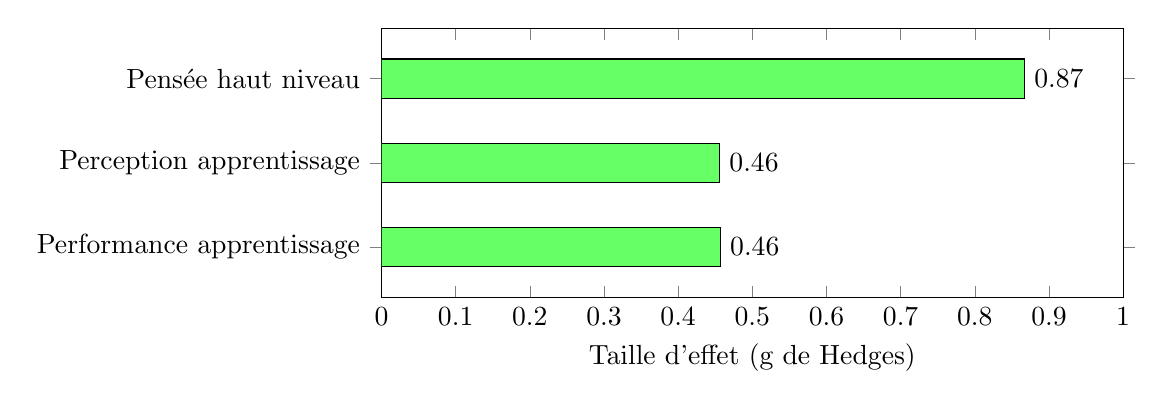
\begin{tikzpicture}
\begin{axis}[
  xbar,
  width=11cm,
  height=5cm,
  xlabel={Taille d'effet (g de Hedges)},
  ytick={1,2,3},
  yticklabels={Performance apprentissage, Perception apprentissage, Pensée haut niveau},
  nodes near coords,
  nodes near coords align={horizontal},
  xmin=0, xmax=1.0,
  bar width=0.5cm,
  enlarge y limits=0.3
]

\addplot[fill=green!60] coordinates {
  (0.867, 3)
  (0.456, 2)
  (0.457, 1)
};

\end{axis}
\end{tikzpicture}
\caption{Tailles d'effet des interventions avec \gls{ia} générative (Wang \& Fan, 2025)}
\label{fig:tailles_effet}
\end{figure}

\medskip

Plus préoccupant, l'étude de Yang et al. (2025) sur 153 lycéens en programmation révèle des effets négatifs significatifs : les groupes utilisant ChatGPT affichent des niveaux plus bas de flow, d'auto-efficacité et de performance comparativement aux méthodes conventionnelles~\cite{yang2025programming}. L'explication avancée repose sur la dépendance excessive : les étudiants consultent ChatGPT au moindre obstacle, ce qui court-circuite l'engagement cognitif profond nécessaire à l'apprentissage durable de la programmation. Les auteurs proposent le modèle G-P-T (Guidance-Practice-Test) pour mitiger ces effets : guidance initiale avec l'\gls{ia}, pratique autonome sans assistance, puis test avec possibilité de recours à l'\gls{ia}. Cette implication est capitale pour Polytech Annecy-Chambéry, où l'enseignement de la programmation occupe une place centrale dans toutes les filières. Deng et al. (2025) confirment dans leur méta-analyse de 69 études expérimentales que, si ChatGPT réduit l'effort mental requis, il n'a \textbf{pas d'effet significatif sur l'auto-efficacité}~\cite{deng2025chatgpt}, ce qui soulève la question des compétences métacognitives et de l'autonomie intellectuelle à long terme.

Un consensus émerge néanmoins sur les conditions de succès. L'apprentissage guidé avec les outils d'\gls{ia} générative produit des résultats supérieurs à l'usage indépendant non encadré. Les effets se révèlent plus importants pour les compétences de bas niveau cognitif — mémorisation, compréhension — que pour les compétences d'ordre supérieur selon la taxonomie de Bloom (analyse, synthèse, évaluation)~\cite{ma2025metaanalysis}. La formation préalable des enseignants et des étudiants aux usages appropriés de l'\gls{ia} constitue un facteur déterminant de succès, confirmant l'importance des dispositifs de formation à la littératie \gls{ia} préconisés par l'\gls{unesco} et le rapport Taddei-Pascal~\cite{batista2024systematic}.

Les documents institutionnels structurent les applications pédagogiques selon deux axes.

\textbf{Pour les enseignants}, le référentiel \gls{unesco} identifie quatre domaines d'application~\cite{unesco2024competences} :

\begin{enumerate}[label=\textbf{\arabic*.}, leftmargin=1.5cm]
  \item \textbf{Préparation de cours et création matériel pédagogique} : Génération d'exercices, scénarios pédagogiques, supports variés.

  \item \textbf{Enseignement assisté et différenciation} : Adaptation contenus selon niveaux, soutien personnalisé aux élèves.

  \item \textbf{Évaluation formative et suivi} : Feedback automatisé, suivi progression, génération grilles évaluation.

  \item \textbf{Recherche} (\gls{inria}) : Aide rédaction articles, amélioration style, traduction contextualisée, génération code~\cite{inria2025note}.
\end{enumerate}

Le gain de temps ainsi libéré peut être réinvesti dans l'accompagnement personnalisé des étudiants, dimension souvent négligée dans l'enseignement supérieur de masse.

\medskip

\textbf{Pour les étudiants}, la charte \gls{insp} précise les usages autorisés~\cite{insp2025charte} :

\begin{enumerate}[label=\textbf{\arabic*.}, leftmargin=1.5cm]
  \item Reformuler un paragraphe avec \textbf{relecture critique obligatoire}
  \item Vérifier le respect d'une consigne
  \item S'entraîner avec des cas pratiques générés
  \item Créer des quiz de révision
  \item Rédiger un \textbf{premier jet à retravailler substantiellement}
\end{enumerate}

\medskip

\noindent\textbf{Frontière claire} : Autonomie renforcée (l'\gls{ia} comme levier d'apprentissage) vs substitution prohibée (l'\gls{ia} comme contournement de l'effort intellectuel)~\cite{men2025cadre}.

Les enquêtes à large échantillon confirment une adoption rapide mais inégalement préparée. Nikolic et al. (2025) interrogent 23~218 étudiants dans 109 pays et documentent les perceptions globales initiales : enthousiasme majoritaire mais inquiétudes persistantes sur l'intégrité académique et l'équité d'accès~\cite{nikolic2025perceptions}. Abbas et al. (2024) conduisent une étude longitudinale sur 494 étudiants en trois vagues de mesure et développent une échelle d'usage validée permettant de distinguer usage superficiel, stratégique et approfondi~\cite{abbas2024harmful}. Le rapport Stanford HAI (2025) révèle un décalage préoccupant : si 81~\% des enseignants en informatique estiment que l'\gls{ia} devrait faire partie de l'éducation fondamentale, moins de 50~\% se sentent équipés pour l'enseigner~\cite{stanford2025aiindex}. Ce besoin massif de formation continue rejoint les préconisations françaises et internationales. Ces usages s'inscrivent désormais dans un cadre réglementaire structuré au niveau européen.

\subsection{Cadre réglementaire et enjeux éthiques}

L'\gls{aiact} (Règlement UE 2024/1689), entré en vigueur en août 2024, constitue le premier cadre juridique complet sur l'intelligence artificielle au monde~\cite{aiact2024}. Son approche par niveau de risque classe l'éducation comme \textbf{secteur à haut risque}, ce qui impose des obligations de conformité aux établissements d'enseignement supérieur. Les pratiques interdites incluent notamment la reconnaissance des émotions sur les lieux de travail et dans les établissements d'enseignement, jugée attentatoire aux libertés fondamentales. Les applications à haut risque comprennent l'accès aux établissements (sélection, orientation), l'évaluation des apprentissages (notation automatisée, détection de fraude) et la surveillance des examens. Cette classification impose une traçabilité des décisions, une évaluation des risques et une possibilité de recours humain. La Commission européenne prépare par ailleurs un AI Literacy Framework pour 2026, définissant les connaissances, compétences et attitudes essentielles pour naviguer dans un environnement saturé d'\gls{ia}. Un fait révélateur motive cette initiative : selon une enquête citée dans le règlement, 48~\% des jeunes de la génération Z déclarent avoir des difficultés à évaluer la fiabilité de l'information générée par l'\gls{ia}. Cette vulnérabilité épistémologique appelle une réponse pédagogique structurée, que Polytech doit anticiper pour ses étudiants ingénieurs.

Les cinq documents convergent vers quatre principes directeurs (Figure~\ref{fig:quatre_principes}).

\begin{figure}[htbp]
\centering
\begin{tikzpicture}[
  principe/.style={rectangle, draw, fill=blue!15, minimum width=3.2cm, minimum height=2.2cm, align=center, font=\small},
  node distance=0.3cm
]
  % 4 boîtes en 2x2
  \node[principe, fill=red!15] (p1) {
    \textbf{1. Responsabilité}\\
    \textbf{humaine}\\[0.3em]
    {\footnotesize L'IA n'est pas}\\
    {\footnotesize un auteur}
  };

  \node[principe, fill=orange!15, right=of p1] (p2) {
    \textbf{2. Transparence}\\
    \textbf{obligatoire}\\[0.3em]
    {\footnotesize Usage explicite}\\
    {\footnotesize et documenté}
  };

  \node[principe, fill=green!15, below=of p1] (p3) {
    \textbf{3. Protection}\\
    \textbf{des données}\\[0.3em]
    {\footnotesize Conformité}\\
    {\footnotesize RGPD}
  };

  \node[principe, fill=purple!15, below=of p2] (p4) {
    \textbf{4. Formation}\\
    \textbf{prérequis}\\[0.3em]
    {\footnotesize Littératie IA}\\
    {\footnotesize indispensable}
  };

  % Titre central
  \node[above=0.8cm of p1.north west, anchor=west, font=\bfseries] {Convergence institutionnelle};
\end{tikzpicture}
\caption{Les quatre principes directeurs identifiés dans les documents institutionnels}
\label{fig:quatre_principes}
\end{figure}

\medskip

Premièrement, la \textbf{responsabilité humaine} : l'\gls{ia} « ne peut pas être considérée comme un auteur » selon l'\gls{inria}, et « chaque usager est pleinement responsable des contenus qu'il produit, même lorsqu'ils sont assistés par une \gls{ia} » selon l'\gls{insp}~\cite{inria2025note,insp2025charte}. Cette responsabilité implique une validation humaine systématique des productions assistées, particulièrement dans des contextes académiques où l'évaluation porte sur le cheminement intellectuel autant que sur le résultat final. Deuxièmement, la \textbf{transparence obligatoire} : le cadre \gls{men} stipule un « usage explicite et assumé », l'\gls{inria} recommande qu'« un guide précis soit élaboré conjointement » par les établissements, et l'\gls{insp} fournit des modèles de citation normalisés, par exemple : « Texte généré avec ChatGPT 4.5, relu et validé par l'auteur le 15/12/2025 »~\cite{men2025cadre,inria2025note,insp2025charte}. Troisièmement, la \textbf{protection des données} conformément au \gls{rgpd} : le \gls{men} précise qu'« aucune donnée confidentielle ou à caractère personnel ne peut être saisie dans les outils \gls{ia} grand public », et l'\gls{insp} liste exhaustivement les données interdites (nom complet, identifiants professionnels, données de santé, opinions politiques)~\cite{men2025cadre,insp2025charte,rgpd2016}. Cet enjeu revêt une acuité particulière pour Polytech Annecy-Chambéry où les projets industriels en partenariat avec des entreprises comportent fréquemment des clauses de confidentialité strictes. Quatrièmement, la \textbf{formation comme prérequis} : le référentiel \gls{unesco} structure 15 compétences sur trois niveaux, le rapport Taddei-Pascal appelle à « former TOUS les étudiants », et l'\gls{inria} recommande des « sessions de formation dans les centres à destination des personnels »~\cite{unesco2024competences,pascal2025ia,inria2025note}. Cette formation à la littératie \gls{ia} devient aussi indispensable que la maîtrise de l'anglais ou des outils numériques de base.

Les cinq documents identifient un ensemble convergent de risques, synthétisé dans le Tableau~\ref{tab:risques_ia}. Les \textbf{hallucinations} (génération de réponses factuellement fausses mais syntaxiquement plausibles) sont mentionnées par l'\gls{unesco}, l'\gls{inria}, le \gls{men} et l'\gls{insp} comme un risque de niveau très élevé. Les \textbf{biais algorithmiques} (reproduction de stéréotypes de genre, ethniques ou sociaux présents dans les données d'entraînement) constituent un risque élevé selon l'\gls{unesco}, le \gls{men} et l'\gls{insp}. La question des \textbf{données personnelles} est jugée critique par l'ensemble des cinq documents. L'\textbf{impact environnemental}, dimension longtemps négligée, est désormais classé comme risque croissant par le rapport Taddei-Pascal, le \gls{men} et l'\gls{insp}. La \textbf{souveraineté numérique} (dépendance vis-à-vis d'acteurs extra-européens) est qualifiée d'enjeu stratégique par le rapport Taddei-Pascal, le \gls{men} et l'\gls{inria}. Enfin, les \textbf{conditions de travail} des annotateurs humains (« travailleurs du clic » dans les pays du Sud) émergent comme risque éthique dans le rapport Taddei-Pascal, le \gls{men} et l'\gls{inria}.

\begin{table}[htbp]
\centering
\caption{Risques identifiés par les documents institutionnels}
\label{tab:risques_ia}
\begin{tabular}{lcc}
\toprule
\textbf{Risque} & \textbf{Documents} & \textbf{Niveau préoccupation} \\
\midrule
Hallucinations & \gls{unesco}, \gls{inria}, \gls{men}, \gls{insp} & Très élevé \\
Biais algorithmiques & \gls{unesco}, \gls{men}, \gls{insp} & Élevé \\
Données personnelles & Tous (5 documents) & Critique \\
Impact environnemental & Taddei-Pascal, \gls{men}, \gls{insp} & Croissant \\
Souveraineté numérique & Taddei-Pascal, \gls{men}, \gls{inria} & Stratégique \\
Conditions de travail & Taddei-Pascal, \gls{men}, \gls{inria} & Émergent \\
\bottomrule
\end{tabular}
\end{table}

\medskip

La charte \gls{insp} fournit les données chiffrées les plus précises sur l'impact environnemental, dimension souvent sous-estimée~\cite{insp2025charte}. Une requête GPT-4 consomme environ 0,32~ml d'eau pour le refroidissement des serveurs, soit l'équivalent énergétique d'une ampoule LED allumée trois minutes. À l'échelle mondiale, avec 2,5 milliards de requêtes par jour pour ChatGPT seul, la consommation atteint 2,9~GWh d'électricité quotidienne et 4 millions de litres d'eau. Ces chiffres, présentés de manière sobre, invitent à une réflexion sur la sobriété numérique sans tomber dans le catastrophisme. L'empreinte carbone doit être mise en perspective avec les bénéfices pédagogiques potentiels, mais elle ne peut être ignorée dans une démarche responsable. Cette dimension émergente mais croissante dans les préoccupations institutionnelles structure les recommandations pour une intégration soutenable de l'\gls{ia} en enseignement supérieur. Ces enjeux éthiques et environnementaux structurent les recommandations institutionnelles.

Les organisations internationales convergent vers des recommandations similaires. L'\gls{unesco} publie en 2023 le premier guide mondial sur l'\gls{ia} générative en éducation et recherche, établissant des principes directeurs : limite d'âge de 13 ans pour l'usage non supervisé, protection des données dans un « sandbox de confidentialité » séparant strictement données de formation et de production, formation obligatoire des enseignants à la littératie \gls{ia}~\cite{unesco2023guidance}. L'approche humaniste de l'\gls{unesco} insiste sur un point central : l'\gls{ia} doit rester au service de l'humain, jamais un substitut, dans une vision où la technologie amplifie les capacités sans remplacer le jugement critique. L'\gls{ocde}, dans ses rapports TALIS et Education Policy Outlook (2024-2025), souligne le potentiel de l'\gls{ia} pour gérer la charge de travail des enseignants par l'automatisation de tâches administratives et le feedback formatif automatisé, tout en alertant sur les défis d'équité et d'inclusion : fracture numérique entre établissements, biais algorithmiques discriminatoires, risque d'accroissement des inégalités~\cite{ocde2024outlook,varsik2024equity,ocde2025teachers}. Le rapport Stanford HAI (2025) confirme le décalage entre l'adhésion de principe (81~\% des enseignants en informatique estiment que l'\gls{ia} devrait faire partie de l'éducation fondamentale) et la préparation effective (moins de 50~\% se sentent équipés pour l'enseigner), révélant un besoin massif de formation continue~\cite{stanford2025aiindex}.

Le rapport Taddei-Pascal structure ses vingt-six recommandations autour de six objectifs, avec un financement estimé entre trois cents et cinq cents millions d'euros sur cinq ans~\cite{pascal2025ia}. Le premier objectif vise à former tous les étudiants à un usage raisonné, durable et éthique de l'\gls{ia}, intégré dans les curricula obligatoires. Le deuxième préconise un grand plan de sensibilisation des personnels enseignants, administratifs et techniques. Le troisième propose le développement de datacenters dédiés à l'inférence souveraine, réduisant la dépendance vis-à-vis des acteurs extra-européens. Le quatrième recommande la labellisation des chartes d'établissement selon le modèle DEMOES (Détermination, Éthique, Mesure, Ouverture, Engagement, Sobriété). Le cinquième appelle à la création d'un Institut national « \gls{ia}, éducation et société » chargé de coordonner la recherche et l'évaluation des pratiques. Le sixième propose l'organisation de conventions citoyennes autour de l'\gls{ia} pour associer la société civile aux décisions stratégiques. La note \gls{inria} formule onze recommandations plus opérationnelles~\cite{inria2025note}, dont l'interdiction de l'utilisation de \gls{llm} pour l'évaluation des candidatures (risque de biais systématiques) et la relecture d'articles scientifiques (conflit avec le principe de responsabilité intellectuelle), la vigilance extrême sur les données confidentielles dans les projets de recherche partenariaux, et la nécessité de développer une « \gls{ia} générative libre et souveraine dédiée au monde de la recherche », alternative aux solutions commerciales extra-européennes. Ce cadre institutionnel et réglementaire pose les fondations d'une gouvernance éthique de l'\gls{ia} en enseignement supérieur, dont les modalités pratiques de mise en œuvre — définition de la fraude académique, protection des données personnelles, impact environnemental — sont examinées en détail dans la section suivante.
